%% Be sure to check spelling!

%% Put **your** name and the proper due date in place

%% Copy the lstlisting and figure code as many times as you need
%% Be sure to put in your own file names if appropriate

%% Note that the \epsfig commands are currently commented out - until the
%%%% files exist, processing this code without them will result in an error
%%%% so leave the comments until you have created the graphics files!

\documentclass{article}
\usepackage{amsmath}    % loads AMS-Math package
\usepackage{epsfig}     % allows PostScript files
\usepackage{listings}   % allows lstlisting environment
\usepackage{moreverb}   % allows listinginput environment
\usepackage{vmargin}    % allows better margins
\setpapersize{USletter} % sets the paper size
\setmarginsrb{1in}{0.5in}{1in}{0.2in}{12pt}{11mm}{0pt}{11mm} %sets margins 
\begin{document}
\begin{center}
\rule{6.5in}{0.5mm}\\~\\
{\bf \large EGR 103L -- Spring 2015}\\~\\
{\huge \bf \LaTeX~Assignment}\\~\\
**NAME (NETID)**\\
Lab Section **NUMBER AND LETTER**, **DAY AND TIMES**\\
**DATEDUE**, **YEAR**\\~\\
{\small I understand and have adhered to all the tenets of the Duke
  Community Standard in completing every part of this assignment.  I
  understand that a violation of any part of the Standard on any part
  of this assignment can result in failure of this assignment, failure
  of this course, and/or suspension from Duke University.} 
%% YOU WILL SIGN THE DOCUMENT HERE
~\\~\\~\\~\\
\rule{6.5in}{0.5mm}\\
\end{center}
\tableofcontents
\listoffigures
\pagebreak

\section{Equations} %%% You will add your equations here
\begin{itemize}
\item General second-order system equation\cite[p.~221]{Rizzoni}:
% unnumbered and aligned equation
\item The Secant Formula for finding maximum stress 
in a column\cite[p.~681]{Hibbeler}:
% unnumbered and aligned equation
\item Characteristic determinant for a 2x2 system of 
differential equations\cite[p.~152]{Kreyszig}:
% aligned numbered equations...except no numbers on first parts
\item Definition of the Lyapunov exponent\cite[p.~56]{Ott}:
% aligned numbered equations
\end{itemize}

\section{Tables using {\tt tabular} and {\tt array}}
\subsection{Using {\tt tabular}} %%% You will add the tabular here
Converting ammonia into nitric acid - the Ostwald Process\cite{Ostwald}:
% centered tabular here
\subsection{Using {\tt array}} %%% You will add the array here
% stretched array here
\pagebreak

\section{Comments} %%% You will add your comments here
Things I learned in this assignment:
% itemized list here


\pagebreak
\appendix
\section{Codes}
%%% Everything in this section is done; make sure you 
%%% understand how it works in general
\subsection{Listing of full sample header for original code}
\listinginput[1]{1}{Header1f.m}

\subsection{Listing of short sample header for original code}
\listinginput[1]{1}{Header1s.m}

\subsection{Listing of full sample header for modified code}
\listinginput[1]{1}{Header2f.m}

\subsection{Listing of short sample header for modified code}
\listinginput[1]{1}{Header2s.m}

\pagebreak
\section{Figures \label{FigureList}}
%%% Almost everything in this section is done; make sure you 
%%% understand how it works in general and be sure to 
%%%uncomment the epsfig lines

\begin{figure}[htb]
\begin{center}
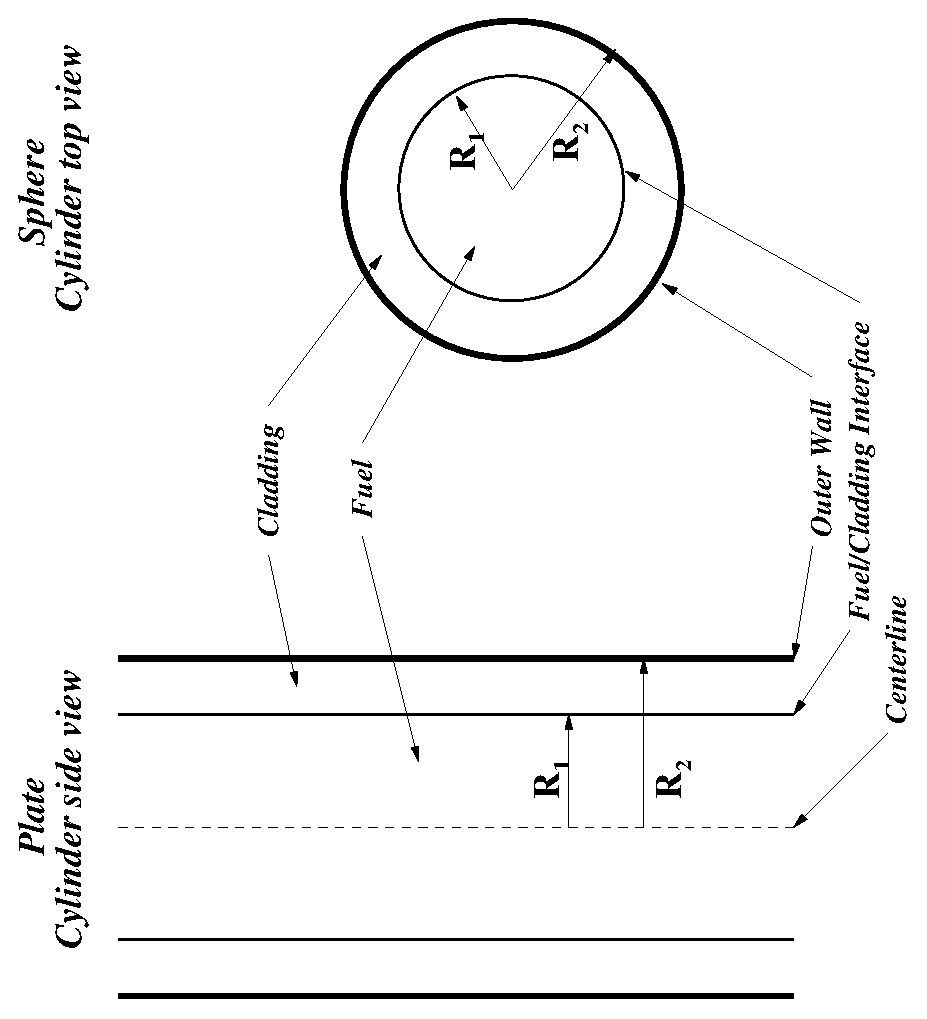
\epsfig{file=drawing.eps, width=3in, angle=-90} 
\caption{Drawing from ME 431L test.}
\end{center}
\end{figure}

\begin{figure}[htb]
\begin{center}
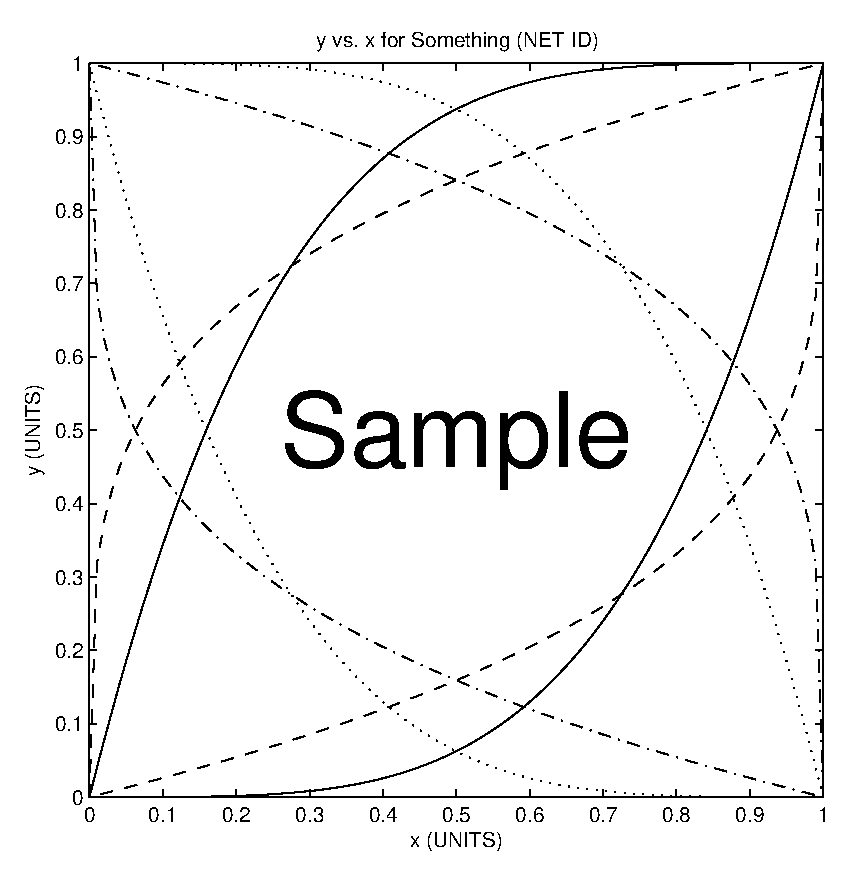
\epsfig{file=SampleFigure.eps, width=2.5in} 
\caption{Sample MATLAB figure.}
\end{center}
\end{figure}
\pagebreak

%%% Everything in this section is done; make sure you 
%%% understand how it works in general
%%% Note that line returns are optional
\addcontentsline{toc}{section}{References}
\begin{thebibliography}{9}
\bibitem{Rizzoni}
Rizzoni, Georgio,
{\it Principles and Applications of Electrical Engineering}.
McGraw-Hill, New York,
5th Edition,
2007.
\bibitem{Hibbeler}
Hibbeler, R. C.,
{\it Mechanics of Materials}.
Pearson Prentice Hall, Upper Saddle River, NJ, 8th Edition, 2011.
\bibitem{Kreyszig}
Kreyszig, Erwin,
{\it Advanced Engineering Mathematics}.
John Wiley \& Sons, New York, 8th Edition, 1999.
\bibitem{Ott}
Ott, Edward,
{\it Chaos in Dynamical Systems}.
Cambridge University Press, Cambridge, UK, 1st Edition, 1993.
\bibitem{Ostwald}
Wikipedia, 
{\it Ostwald process} (http://en.wikipedia.org/wiki/Ostwald$\_$process).
Online; accessed 19-Aug-2012.
\end{thebibliography}

\end{document}
